%%=====================================================================
%% RESULTADOS
%% Slides com \ilustrativo trazem dados provisórios: substituir.
%%=====================================================================
\secaoudesc{Resultados}

\begin{frame}{Parâmetros elétricos}
  \begin{columns}[c]
    \begin{column}{0.5\textwidth}
      \begin{itemize}
        \item Resistência por quatro fios (Kelvin)
        \item Indutância por ressonância LC
        \item Ensaios independentes convergentes
      \end{itemize}
    \end{column}
    \begin{column}{0.5\textwidth}
      \centering
      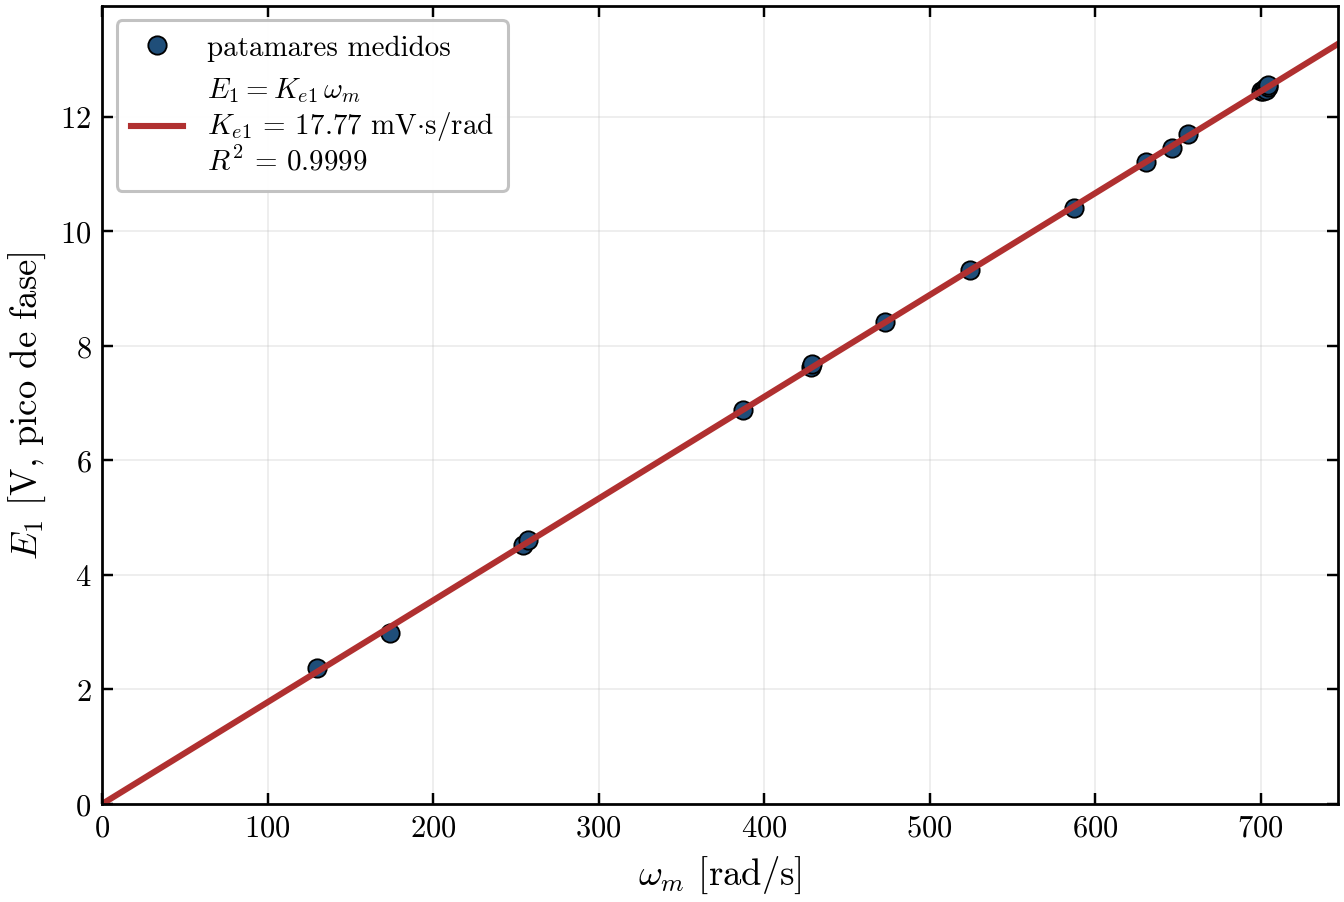
\includegraphics[width=\linewidth]{Resultados/bancada_ke.png}
      \fonte[Autor; Fitzgerald, Kingsley e Umans (2014)]
    \end{column}
  \end{columns}
\end{frame}

\begin{frame}{Perdas mecânicas}
  \begin{columns}[c]
    \begin{column}{0.36\textwidth}
      \begin{itemize}
        \item Ensaio em vazio
        \item Balanço de potência por fase
        \item Atrito viscoso e seco
      \end{itemize}
    \end{column}
    \begin{column}{0.64\textwidth}
      \centering
      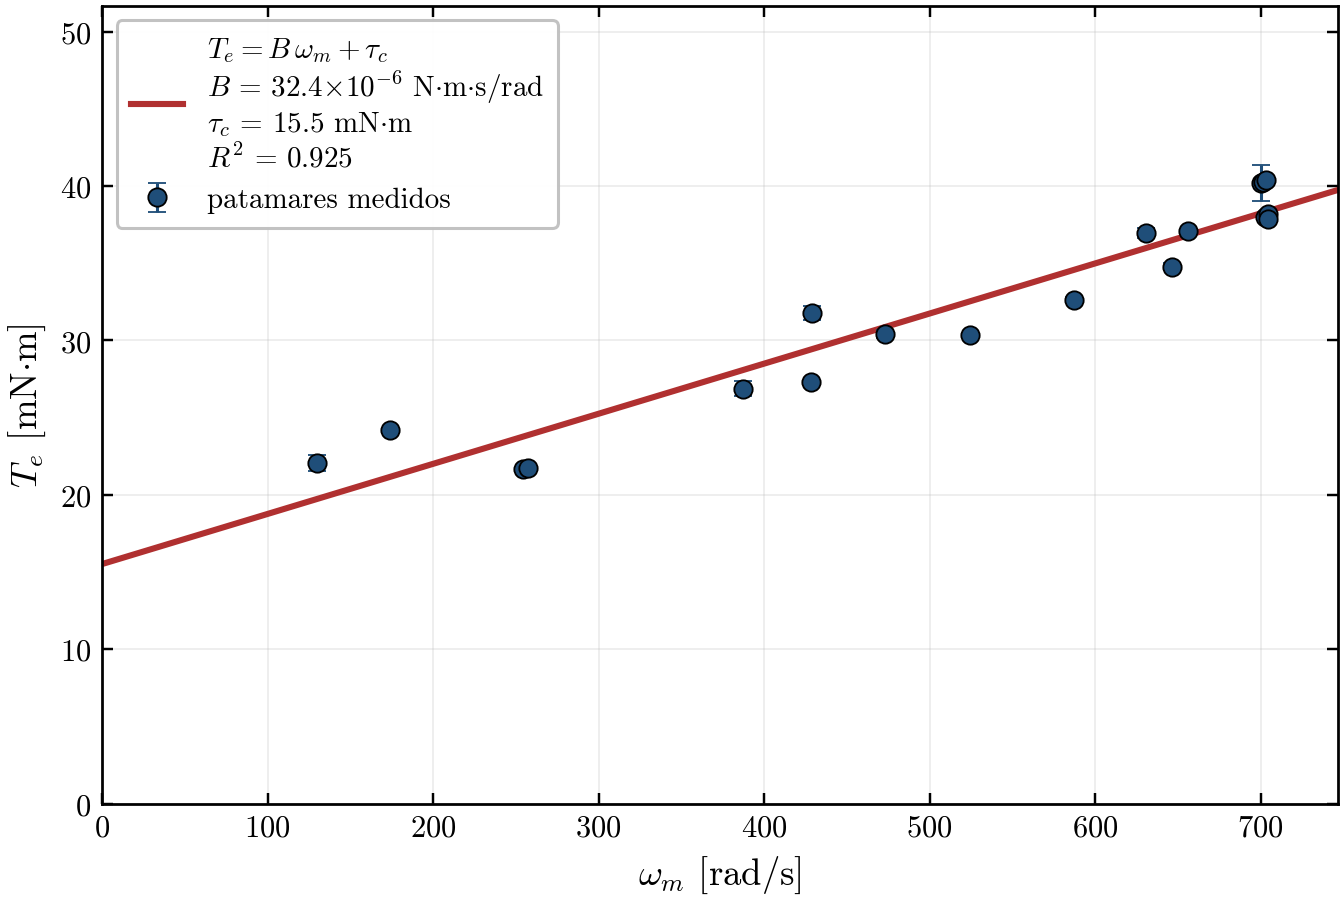
\includegraphics[width=\linewidth]{Resultados/bancada_te_omega.png}
      \fonte[Autor; Krishnan (2017)]
    \end{column}
  \end{columns}
\end{frame}

\begin{frame}{Observador em bancada}
  \begin{columns}[c]
    \begin{column}{0.36\textwidth}
      \begin{itemize}
        \item Rotação acompanha o tacômetro
        \item Ângulo coerente com os pulsos
        \item Limite em baixa rotação
      \end{itemize}
    \end{column}
    \begin{column}{0.64\textwidth}
      \centering
      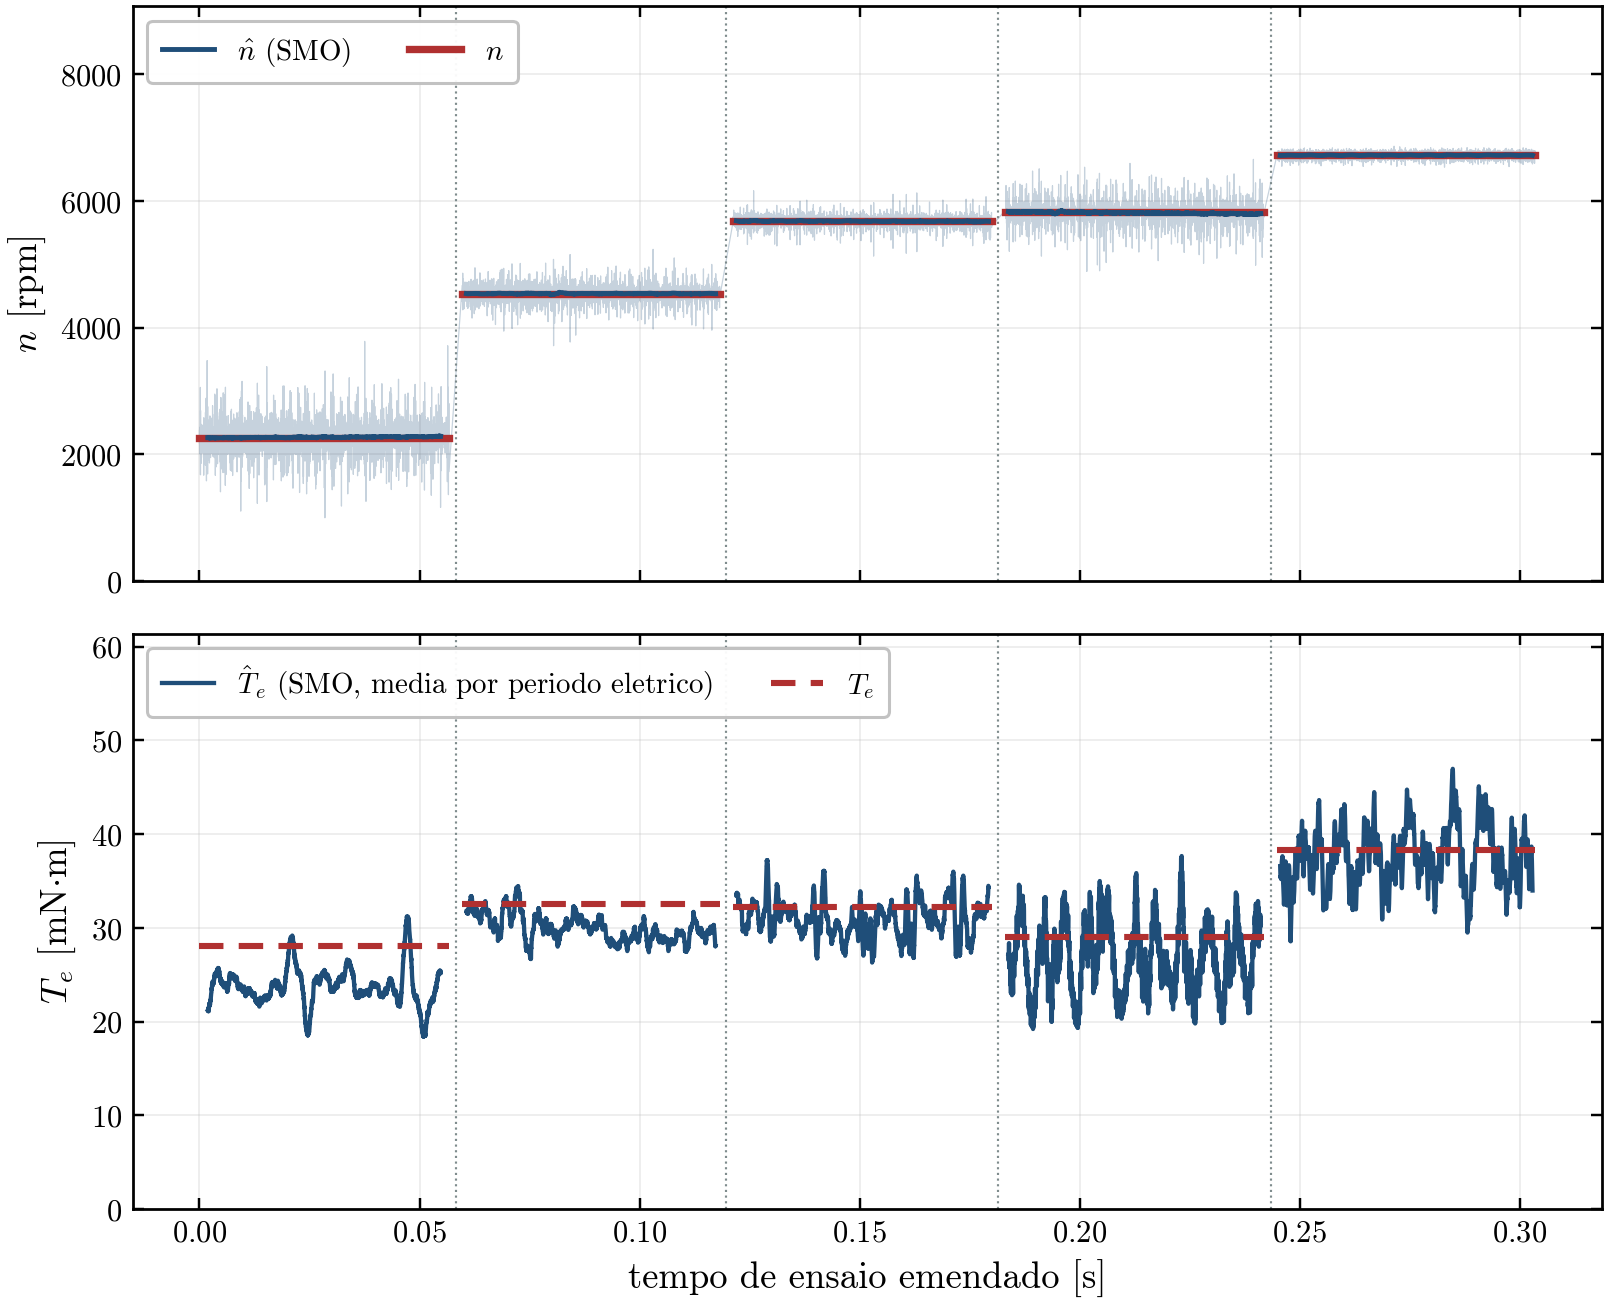
\includegraphics[height=0.72\textheight]{Resultados/bancada_smo_rpm_torque.png}
      \fonte[Autor; Nidec (2026)]
    \end{column}
  \end{columns}
\end{frame}

\begin{frame}{Torque da hélice}
  \begin{columns}[c]
    \begin{column}{0.36\textwidth}
      \begin{itemize}
        \item Duas hélices APC
        \item $C_Q$ estimado só com grandezas elétricas
        \item Comparado ao fabricante
      \end{itemize}
    \end{column}
    \begin{column}{0.64\textwidth}
      \centering
      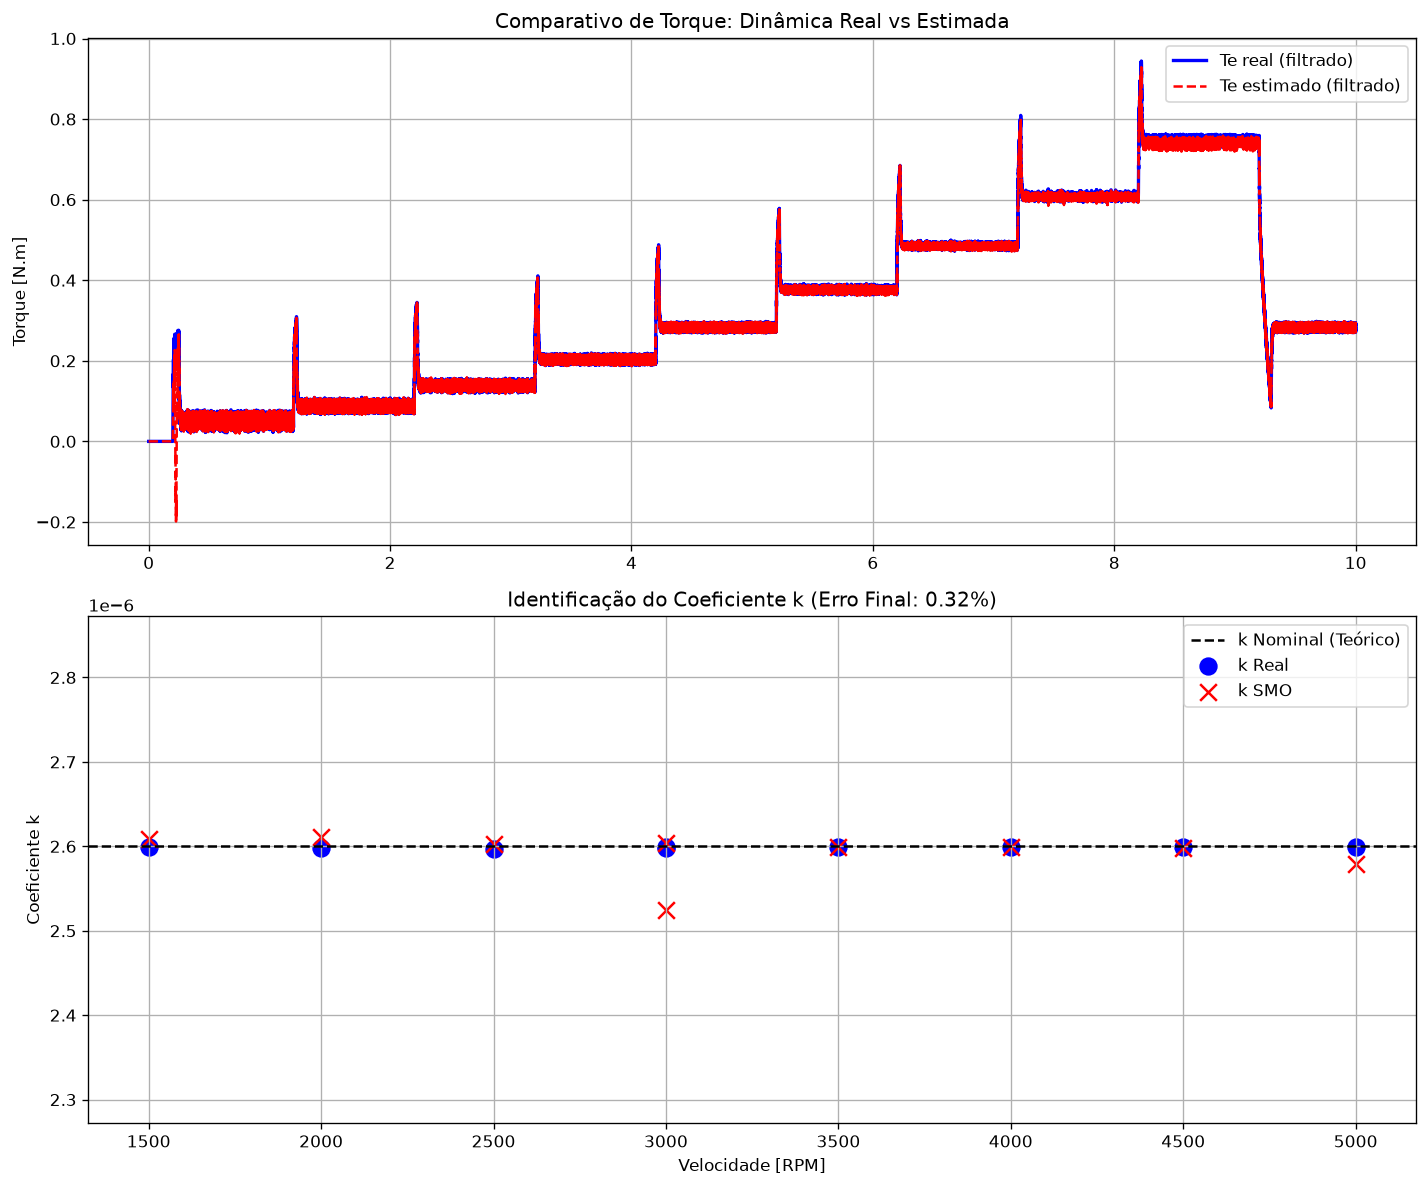
\includegraphics[height=0.72\textheight]{Desenvolvimento/Algortimo_Coeficiente_helice_17x10E.png}
      \fonte[Autor; APC Propellers (2026); Selig (2026); McCormick (1995)]
    \end{column}
  \end{columns}
\end{frame}

%% ----- a partir daqui: RESULTADOS ILUSTRATIVOS (substituir) -----

\begin{frame}{Validação da SIBA}
  \ilustrativo
  \centering
  \begin{tabular}{lc}
    \toprule
    \textbf{Sensor} & \textbf{Erro vs. referência} \\
    \midrule
    Tensão da bateria   & Dentro da tolerância \\
    Corrente da bateria & Dentro da tolerância \\
    Células de carga    & Dentro da tolerância \\
    Tubo de Pitot       & Dentro da tolerância \\
    \bottomrule
  \end{tabular}
  \fonte[Autor; Northrup (2018); Brandt et al.\ (2015)]

  \destaque{Cadeia aerodinâmica dentro da faixa exigida pela equipe.}
\end{frame}

\begin{frame}{Ensaio integrado}
  \ilustrativo
  \begin{columns}[c]
    \begin{column}{0.36\textwidth}
      \begin{itemize}
        \item SIBA e SAME sincronizadas
        \item Tração, torque e rotação no mesmo registro
        \item Exportação em CSV
      \end{itemize}
    \end{column}
    \begin{column}{0.64\textwidth}
      \centering
      \placeholder{8.5cm}{5.2cm}{Tração e torque estimado\\em função da rotação\\(ensaio integrado)}
      \fonte
    \end{column}
  \end{columns}
\end{frame}
